\section*{Question 3}
\fakesection{3}

This problem revisits the polyphase interpolator of Question 2, but with the additional task of heterodyning with a 10 kHz carrier. This is easily achieved with one extra step. After zero-padding and reshaping the filter coefficients into a matrix, we multiply each row by
\begin{align}
    c(n) = \cos(2\pi nk/L),\ n = 0 \dots L-1
\end{align}
where $L$ is the upsampling factor, $n$ is the row index, and $k$ is a shifting constant:
\begin{align}
    k = L \cdot \frac{f_c}{f_s}
\end{align}
Here, $f_c$ is the carrier frequency, 10 kHz, and $f_s$ is the frequency after upsampling, 40 kHz. Applying the filter the same way as for Question 2, the input signal is simultaneously upsampled, filtered and frequency shifted. Figure \ref{fig:q3_heterodyne} shows the output.

\begin{figure}[ht]
    \centering
    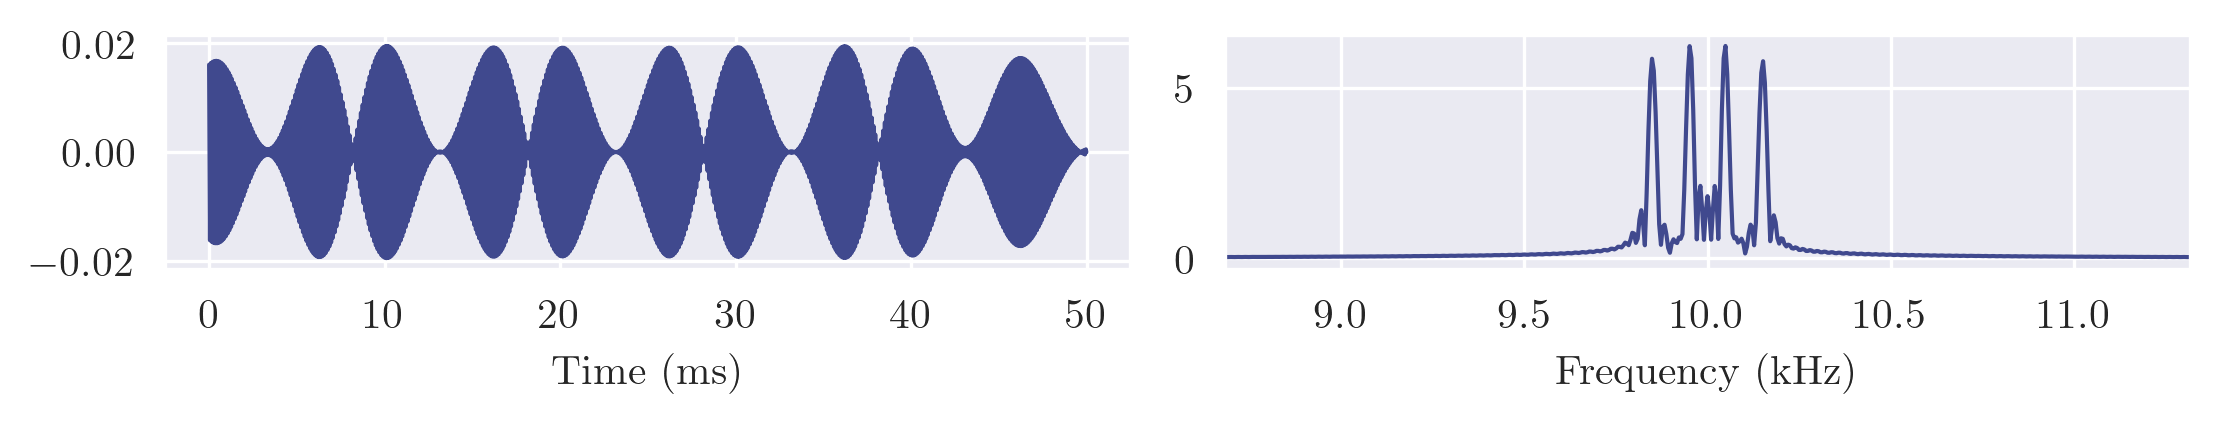
\includegraphics[width=\textwidth]{images/q3_heterodyne.png}
    \caption{Simultaneous heterodyning with 10 kHz carrier by polyphase interpolator}
    \label{fig:q3_heterodyne}
\end{figure}

To see how much overhead is added, we time 10,000 trials and compare the result with those from Question 2. The average time per trial is 0.801 ms. This is equal to the timing without heterodyning (to the presented precision), though typically we would expect some variance. Hence, we have achieved heterodyning without incurring significant additional computation.
